%!TEX root = ../main.tex
\section{Design}
\subsection{MicroZed Carrier Card}
\label{sub:microzed_carrier_card}
Avnet supplies a MicroZed breakout carrier card as a reference design for designing carrier cards.
All of the schematics and layout documents are made publicly available and will, in conjunction with the carrier card design guide \cite{design_carrier} form the basis for the design of the swarmbot carrier card.

\subsubsection*{Power Requirements}
\label{sub:power_req}
A carrier card  needs to provide the following voltages for the MicroZed:
\begin{itemize}
	\item $V_{in} = 5V$
	\item $V_{ccio,13}$ (Voltage logic level for I/O bank 13)
	\item $V_{ccio,34}$ (Voltage logic level for I/O bank 34)
	\item $V_{ccio,35}$ (Voltage logic level for I/O bank 35)
\end{itemize}
The different I/0 banks can be operated at different voltage levels.
According to \cite{zynq_dc}, the possibly logic levels are 1.2V, 1.5V, 1.8V, 2.5V, and 3.3V.

It was chosen to supply all I/O banks with a voltage level of 3.3V as the vast majority of hardware used at the hardware is available at this voltage.
Additionally, it simplifies both the circuitry, as well as the use of the board.

$$ V_{ccio} =  V_{ccio,13} = V_{ccio,34} = V_{ccio,35} = 3.3V$$

The generation of the 3.3V rail is defined in \cite{carrier_schematic} and will be discussed in more detail in section \ref{sec:33v}.
Since the swarmbot is designed to be powered from a 7.4V LiPo battery, the 5V rail has to be generated from this rail.
As the voltage of a battery is not static, the converter will have to be able to supply the required voltage throughout the entire discharge cycle.
\thomas{Is the battery mentioned?}
\thomas{Add figure on discharge curve.}
As can be seen on figure \ref{fig:discharge}, the maximum voltage once fully charged is 8.4V while the minimum voltage when discharged is 6.3V.
\thomas{Check min and max voltages fit discharge curve.}
\begin{figure}
	\centering
	% This file was created by matlab2tikz.
%
\definecolor{mycolor1}{rgb}{0.00000,0.44700,0.74100}%
\definecolor{mycolor2}{rgb}{0.85000,0.32500,0.09800}%
\definecolor{mycolor3}{rgb}{0.92900,0.69400,0.12500}%
\definecolor{mycolor4}{rgb}{0.49400,0.18400,0.55600}%
%
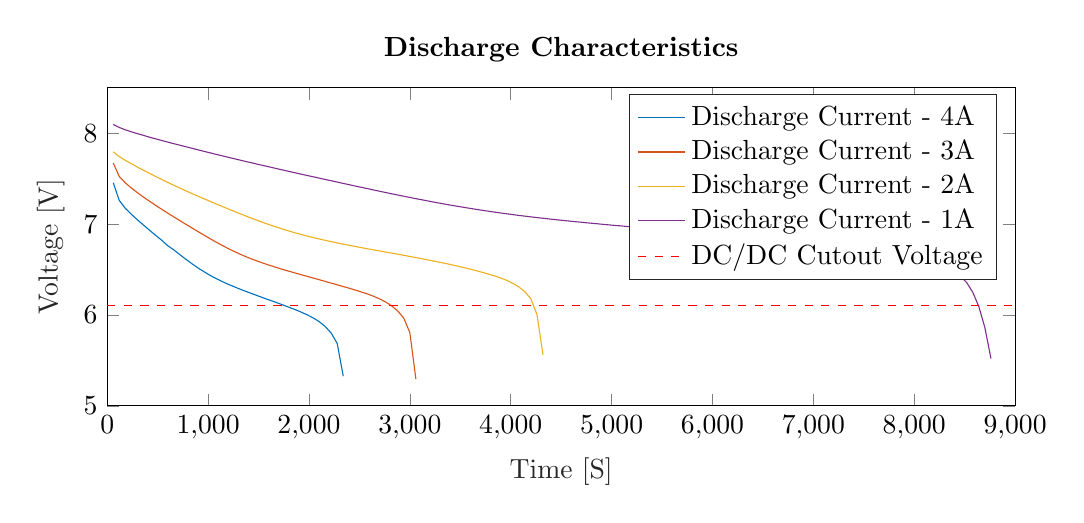
\begin{tikzpicture}

\begin{axis}[%
width=0.951\linewidth,
height=0.333\linewidth,
at={(0\linewidth,0\linewidth)},
scale only axis,
xmin=0,
xmax=9000,
xlabel style={font=\color{white!15!black}},
xlabel={Time [S]},
ymin=5,
ymax=8.5,
ylabel style={font=\color{white!15!black}},
ylabel={Voltage [V]},
axis background/.style={fill=white},
title style={font=\bfseries},
title={Discharge Characteristics},
legend style={legend cell align=left, align=left, draw=white!15!black}
]
\addplot [color=mycolor1]
  table[row sep=crcr]{%
60	7.456\\
120	7.26\\
180	7.174\\
240	7.108\\
300	7.047\\
360	6.99\\
420	6.933\\
480	6.877\\
540	6.823\\
600	6.763\\
660	6.717\\
720	6.664\\
780	6.613\\
840	6.564\\
900	6.518\\
960	6.476\\
1020	6.436\\
1080	6.401\\
1140	6.368\\
1200	6.338\\
1260	6.31\\
1320	6.283\\
1380	6.257\\
1440	6.233\\
1500	6.208\\
1560	6.183\\
1620	6.16\\
1680	6.136\\
1740	6.111\\
1800	6.086\\
1860	6.06\\
1920	6.033\\
1980	6.003\\
2040	5.969\\
2100	5.928\\
2160	5.874\\
2220	5.801\\
2280	5.687\\
2340	5.326\\
};
\addlegendentry{Discharge Current - 4A}

\addplot [color=mycolor2]
  table[row sep=crcr]{%
60	7.673\\
120	7.524\\
180	7.454\\
240	7.397\\
300	7.346\\
360	7.297\\
420	7.252\\
480	7.207\\
540	7.164\\
600	7.121\\
660	7.08\\
720	7.039\\
780	6.998\\
840	6.958\\
900	6.918\\
960	6.879\\
1020	6.84\\
1080	6.802\\
1140	6.766\\
1200	6.731\\
1260	6.699\\
1320	6.668\\
1380	6.639\\
1440	6.613\\
1500	6.588\\
1560	6.565\\
1620	6.543\\
1680	6.522\\
1740	6.501\\
1800	6.482\\
1860	6.463\\
1920	6.444\\
1980	6.426\\
2040	6.407\\
2100	6.389\\
2160	6.37\\
2220	6.351\\
2280	6.332\\
2340	6.313\\
2400	6.294\\
2460	6.274\\
2520	6.253\\
2580	6.231\\
2640	6.206\\
2700	6.177\\
2760	6.143\\
2820	6.1\\
2880	6.044\\
2940	5.965\\
3000	5.806\\
3060	5.294\\
};
\addlegendentry{Discharge Current - 3A}

\addplot [color=mycolor3]
  table[row sep=crcr]{%
60	7.796\\
120	7.743\\
180	7.702\\
240	7.665\\
300	7.628\\
360	7.593\\
420	7.559\\
480	7.525\\
540	7.492\\
600	7.46\\
660	7.428\\
720	7.397\\
780	7.367\\
840	7.337\\
900	7.308\\
960	7.279\\
1020	7.251\\
1080	7.222\\
1140	7.195\\
1200	7.167\\
1260	7.14\\
1320	7.113\\
1380	7.087\\
1440	7.061\\
1500	7.037\\
1560	7.012\\
1620	6.989\\
1680	6.967\\
1740	6.945\\
1800	6.925\\
1860	6.905\\
1920	6.887\\
1980	6.869\\
2040	6.853\\
2100	6.837\\
2160	6.822\\
2220	6.807\\
2280	6.793\\
2340	6.779\\
2400	6.767\\
2460	6.754\\
2520	6.741\\
2580	6.729\\
2640	6.717\\
2700	6.705\\
2760	6.693\\
2820	6.681\\
2880	6.669\\
2940	6.657\\
3000	6.644\\
3060	6.632\\
3120	6.619\\
3180	6.606\\
3240	6.593\\
3300	6.579\\
3360	6.566\\
3420	6.551\\
3480	6.536\\
3540	6.52\\
3600	6.504\\
3660	6.487\\
3720	6.469\\
3780	6.45\\
3840	6.43\\
3900	6.407\\
3960	6.381\\
4020	6.349\\
4080	6.309\\
4140	6.257\\
4200	6.176\\
4260	6.005\\
4320	5.562\\
};
\addlegendentry{Discharge Current - 2A}

\addplot [color=mycolor4]
  table[row sep=crcr]{%
60	8.097\\
120	8.064\\
180	8.038\\
240	8.016\\
300	7.996\\
360	7.977\\
420	7.957\\
480	7.939\\
540	7.921\\
600	7.903\\
660	7.886\\
720	7.869\\
780	7.852\\
840	7.835\\
900	7.818\\
960	7.801\\
1020	7.785\\
1080	7.768\\
1140	7.752\\
1200	7.736\\
1260	7.72\\
1320	7.704\\
1380	7.688\\
1440	7.673\\
1500	7.657\\
1560	7.642\\
1620	7.627\\
1680	7.611\\
1740	7.596\\
1800	7.581\\
1860	7.566\\
1920	7.551\\
1980	7.536\\
2040	7.522\\
2100	7.507\\
2160	7.492\\
2220	7.478\\
2280	7.463\\
2340	7.448\\
2400	7.434\\
2460	7.419\\
2520	7.405\\
2580	7.391\\
2640	7.376\\
2700	7.362\\
2760	7.348\\
2820	7.334\\
2880	7.321\\
2940	7.307\\
3000	7.294\\
3060	7.28\\
3120	7.268\\
3180	7.255\\
3240	7.242\\
3300	7.23\\
3360	7.218\\
3420	7.206\\
3480	7.195\\
3540	7.184\\
3600	7.173\\
3660	7.162\\
3720	7.152\\
3780	7.142\\
3840	7.132\\
3900	7.123\\
3960	7.114\\
4020	7.105\\
4080	7.096\\
4140	7.088\\
4200	7.08\\
4260	7.072\\
4320	7.065\\
4380	7.057\\
4440	7.05\\
4500	7.043\\
4560	7.036\\
4620	7.029\\
4680	7.023\\
4740	7.016\\
4800	7.01\\
4860	7.004\\
4920	6.997\\
4980	6.991\\
5040	6.985\\
5100	6.98\\
5160	6.973\\
5220	6.968\\
5280	6.962\\
5340	6.956\\
5400	6.95\\
5460	6.945\\
5520	6.939\\
5580	6.934\\
5640	6.928\\
5700	6.923\\
5760	6.917\\
5820	6.912\\
5880	6.907\\
5940	6.901\\
6000	6.896\\
6060	6.89\\
6120	6.885\\
6180	6.879\\
6240	6.873\\
6300	6.868\\
6360	6.863\\
6420	6.857\\
6480	6.851\\
6540	6.846\\
6600	6.84\\
6660	6.834\\
6720	6.828\\
6780	6.821\\
6840	6.816\\
6900	6.809\\
6960	6.803\\
7020	6.796\\
7080	6.789\\
7140	6.782\\
7200	6.774\\
7260	6.766\\
7320	6.758\\
7380	6.75\\
7440	6.741\\
7500	6.731\\
7560	6.72\\
7620	6.709\\
7680	6.697\\
7740	6.684\\
7800	6.67\\
7860	6.655\\
7920	6.64\\
7980	6.626\\
8040	6.611\\
8100	6.595\\
8160	6.577\\
8220	6.558\\
8280	6.535\\
8340	6.508\\
8400	6.474\\
8460	6.426\\
8520	6.356\\
8580	6.25\\
8640	6.092\\
8700	5.86\\
8760	5.52\\
};
\addlegendentry{Discharge Current - 1A}

\addplot [color=red, dashed]
  table[row sep=crcr]{%
0	6.1\\
9000	6.1\\
};
\addlegendentry{DC/DC Cutout Voltage}

\end{axis}
\end{tikzpicture}%
	\caption{Discharge curve of the Ansmann 18650 2S1P Li-Ion battery used to power the swarmbot.}
	\label{fig:discharge}
\end{figure}
According to \cite{microzed_hardware_guide} the estimated maximum power draw of the MicroZed is 1.7A at 5V.
This is assuming 85\% utilisation of PL and a conservative 80\% efficiency of the converters.
The estimate made by Avnet is made with the Zynq-7010 in the Xilinx Power Estimator (XPE) \cite{xpe}.
The MicroZed used for the swarmbot project, however, is equipped with the Zynq-7020, a slightly larger chip.
Running the same scenario, 85\% utilisation, in XPE reveals that the 7020 draws 2.3W, just 0.1W more than the 7010, a marginal difference in the total power budget.
In addition to the MicroZed, also the debug LEDs and the microphone board are powered from this rail, adding an estimated $\approx$150mA extra current draw.
In summary, these are the requirements for the DC/DC converter used for generating the 5V rail:

\begin{itemize}
	\item Must function across the entire voltage range of the battery, 6.5V to 8.4V.
	\item Should be able to supply at least 1.85A at 5V.
\end{itemize}

Below is a discussion of the various choices made in the design of the circuitry of the 5V supply.

\paragraph{Designing the 5V Rail}
The PTH08080WAH \cite{pth08080} meets these requirements at a maximum power delivery of 2A/10W/5V.
The device is designed to have a wide input range, accepting \texttt{Vin}=\texttt{Vo}+1.1V to 18V.
At the required 5V this translates to an input range of 6.1V to 18V.
\texttt{Vo} is determined via an external resistor \texttt{Rset}.
A formulae is provided to calculate the exact \texttt{Rset} needed for a given voltage, however a large table of common values is already calculated.
According to this table, \texttt{Rset}=353$\omega$ results in 5V.
353$\omega$ is not a standard value, choosing 348$\omega$ instead yields 5.01V, which is fine for this application.
\\~\\
The circuit appertaining to this component can be seen in figure \ref{fig:dcdccomponent}.
This is the standard application circuit as shown in the datasheet (figure 10 \cite{pth08080}).
According to the datasheet, the minimum recommended input capacitance is 100$\mu$F. 
Of the capacitors on the list of recommended capacitors, also given in the datasheet, the 20SVP150M was chosen.
It is rated for 20V, sufficient for this application, and has a capacitance of 150$\mu$F. 

\begin{figure}
	\centering
	\includegraphics[width=\linewidth]{graphics/5v}
	\caption{Circuit for generating \texttt{VCC}, the 5V rail.}
	\label{fig:pth08080}
\end{figure}

\subsubsection*{Power Up Sequencing}
On power up the first that needs to happen is to pull the MicroZeds PWR\_EN high on the carrier card.
This is done with a pull-up resistor as shown in figure \ref{fig:pwr_en_circuit}.

\begin{figure}
	\centering
	\includegraphics[width=.4\linewidth]{graphics/power_en_sch.pdf}
	\caption{Circuit for proper power sequencing on MicroZeds PWR\_EN.}
	\label{fig:pwr_en_circuit}
\end{figure}

When the MicroZed has powered up its internal DC/DC converters and is ready to receive voltage on its I/O banks the VCCIO\_EN will go high.
VCCIO\_EN has a logic level of 1.8V and the signal is therefore fed to a comparator that outputs a 5V signal to a DC/DC converter when VCCIO\_EN is high.
The DC/DC converter is configured to produce a voltage level of 3.3V that is connected to $V_{ccio}$
This circuitry can be seen in figure \ref{fig:pwr_io_circuit}.

\begin{figure}
	\centering
	\includegraphics[width=1\linewidth]{graphics/vccio_power_up.pdf}
	\caption{Circuit for proper power sequencing on I/O banks.}
	\label{fig:pwr_io_circuit}
\end{figure}

\subsubsection*{Power Down Sequencing}
On power down VCCIO\_EN, DCDC\_EN and PWR\_EN should be pulled down. 
VCCIO\_EN needs to be pulled down first, hereafter PWR\_EN and lastly DCDC\_EN .
The signals are pulled down by MOSFETS controlled by the V\_OFF signal.
When the power switch on the carrier card is flicked, the battery voltage is connected to the V\_OFF rail thereby turning the MOSFETS on and pulling the signals down. 
The correct sequence is maintained by charging capacitors on the gate side of the MOSFETS thereby creating a delay.
Such a MOSFET circuit is shown in figure \ref{fig:pwr_en_circuit}.


\begin{table}

\centering
\caption{My caption}
\label{my-label}
\begin{tabular}{|p{0.5cm}|p{2cm}|p{1.5cm}|l|l|p{5cm}|}
\hline
\#      & Component              & Quantity & MicroZed Carrier Card & SwarmBot Carrier Card & Comment                                                                                                                                                                                                      \\ \hline
1       & Capacitor              & 7        & 0805ZD226MAT2A        & GRM21BR60J226ME39L    & Found equivalent capacitor as the original comes in packages of 3000.                                                                                                                                        \\ \hline
2       & DNP                    &          &                       &                       &                                                                                                                                                                                                              \\ \hline
3       & Capacitor              & 8        & 06035C104KAT2A        & GCM21BR71H104KA02L    & Found equivalent capacitor with 0805 footprint                                                                                                                                                               \\ \hline
4       & Capacitor              & 4        & 04023C104KAT2A        & C0805C103K5RACTU      & Original was out of stock. Found equivalent capacitor with 0805 footprint                                                                                                                                    \\ \hline
5       & Connector              &          &                       &                       & Equivalent ones will be found at the component storage at SDU                                                                                                                                                \\ \hline
6       & MicroUSB               & 1        & 1981584-1             & 47589-0001            & Original needs to be bought in packs of 10. Found a cheaper equivalent one that can be bought in packs of 5.                                                                                                 \\ \hline
7       & DNP                    &          &                       &                       &                                                                                                                                                                                                              \\ \hline
8       & Schottky Diode         & 1        & MBR230LSFT1G          & SBR2A40P1-7           & Original only ships in packs of 50. Found a a similiar diode with. Has a a higher forward voltage drop, but rough calculations estimate that it will only decrease the efficiency with one percentage point. \\ \hline
9       & Schottky Diode         & 2        & BAT54LT1G             & SBR2A40P1-7           & The SBR2A40P1-7 diode is better in all aspects and 25 of them are already bought for \#8                                                                                                                     \\ \hline
10      & Jumper                 &          & 969102-0000-DA        &                       & Is not needed on the SwarmBot Carrier Card.                                                                                                                                                                  \\ \hline
11      & Connector              &          & 5-146257-3            &                       & Is not needed on the SwarmBot Carrier Card.                                                                                                                                                                  \\ \hline
12      & Bergstak connector     & 2        & 61083-104400LF        & 61083-104400LF        &                                                                                                                                                                                                              \\ \hline
13      & Inductor               & 1        & SRN5020-2R2Y          & SRN5020-2R2Y          &                                                                                                                                                                                                              \\ \hline
14      & DNP                    &          &                       &                       &                                                                                                                                                                                                              \\ \hline
\end{tabular}	
\end{table}

\begin{table}
\centering
\caption{My caption}
\label{my-label}
\begin{tabular}{|p{0.5cm}|p{2cm}|p{1.5cm}|l|l|p{5cm}|}
\hline

15      & MOSFET                 & 2        & BSS138LT1G            & BSS138LT1G            &                                                                                                                                                                                                              \\ \hline
16 - 32 & Resistors              &          &                       &                       & Equivalent ones will be found at the component storage at SDU                                                                                                                                                \\ \hline
33      & Converter              & 1        & LMR10510XMFE/NOPB     & LMR10510XMFE/NOPB     &                                                                                                                                                                                                              \\ \hline
34      & Switch                 & 1        & 1101-M2-S3-C-Q-E-2    &  1101M2S3CQE2         &                                                                                                   \\ \hline
35      & DNP                    &          &                       &                       &                                                                                                                                                                                                              \\ \hline
36      & Comparator             & 1        & AP331AWG-7            & LMV331QDBVRQ1         & Original ships in packs of 50. New comparator is compatible, faster and ships in packs of 5.                                                                                                                 \\ \hline
37      & Programmable reference & 1        & TL431AIDBZR           & TL431AIDBZR           &                                                                                                                                                                                                              \\ \hline
x      & Capacitor for anti-aliasing filter  & 4        & NA           & 08055C102KAT2A           &  Similar to the one used in the MicroZed I/O carrier card and with the 0805 footprint                                                                                                                                                                                                      \\ \hline
x      & Resistors for anti-aliasing fitler  & 8        & NA           &            &  SDUs storage                                                                                                                                                                                                     \\ \hline


\end{tabular}

	
\end{table}
